\documentclass{article}
\usepackage[pdftex]{graphicx}
\usepackage{amsmath}
\author{Michael Anderson}
\title{Homework Set 2}
\begin{document}
\maketitle
\center{CS531}
\center{Prof. Tadepalli}\\
\flushleft
\begin{enumerate}
\item[\textbf{3.5}] There are n ways to place the queen in the first column, and that queen can attack
at most 3 squares in the second column. So for each placement of a queen in the first column
there are at least $n-3$ possible placements of the queen in the second column. That second
queen attacks at most 3 more squares in the third column, so for each of the queen placements
in the first and second columns there are at most n-6 placements of the queen in the third
column.

Given this, it is trivial to see that a lower bound for the total number of possible placements
of n queens on an $n \times n$ board is $n(n-3)(n-6)(n-9) \ldots (1or2or3)$.

Since $(n)^3(n-3)^3(n-6)^3(n-9)^3 \ldots (1or2or3)^3$ is on the order of but also greater than 
$(n)(n-1)(n-2)(n-3)(n-4) \ldots (1)=n!$, this result is lower bounded by $\sqrt[3]{n!}$

Suppose that adding a queen takes on average 1000 clock cycles on a typical computer. Modern
desktops have processors that run on the order of a few billion clock cycles per second. So
adding more than a billion queens will probably incur a significant delay. Since
$\sqrt[3]{26!} < 10^9 < \sqrt[3]{27!}$, it is not feasible to solve this problem for values of
n much greater than 27 using exhaustive search. n = 50 would take roughly $10^{25}$ cycles.

\item[\textbf{3.6}]
% Formulation parts: states, Initial state, actions, transition model, goal test, path cost
\begin{enumerate}
\item[a)]
\emph{States}: Each region of the map is either uncolored or has one of four colors.\\
\emph{Initial State:} All regions of the map are uncolored.\\
\emph{Actions:} One region is colored, is uncolored, or changes color.\\
\emph{Transition Model:} Each action changes the state of a region.\\
\emph{Goal Test:} All regions are colored and no region shares a color with any of its neighbors.\\
\item[b)]
\emph{States:} The location of the crates on the floor, whether they are stacked or not, whether the monkey
is standing on the crates or the floor.\\
\emph{Initial State:} Both crates and the monkey are standing on the floor, for example.\\
\emph{Actions:} Push crates around the floor, stack crates, unstack crates, climb onto a crate, climb off of a crate,
grab bananas if they are in reach.\\
\emph{Transition model:} Pushing, stacking, and unstacking crates changes their location; climbing up and down a
crate changes the monkey's location.\\
\emph{Goal Test:} The monkey is able to grab the bananas.\\
\item[c)]
\emph{States:} Each record is either processed or unprocessed, and the program is outputting the message or is not.\\
\emph{Initial State:} All records are unprocessed.\\
\emph{Actions:} Process one of the unprocessed records.\\
\emph{Transition model:} Each action changes one of the records from unprocessed to processed, and may cause the
program to output the message.\\
\emph{Goal Test:} Program outputs the message.\\
\item[d)]
\emph{States:} Each jug contains some positive integer number of gallons of water, that does not exceed their maximum
capacity.\\
\emph{Initial State:} All jugs are empty.\\
\emph{Actions:} Fill a jug from the faucet, use a jug to fill another jug, empty a jug into another jug, empty a jug onto the ground.\\
\emph{Transition model:} Actions change the number of gallons of water in either one or two jugs.\\
\emph{Goal Test:} One of the jugs contains 1 gallon of water.\\
\end{enumerate}

\item[\textbf{3.8}]
\begin{enumerate}
\item[a)]
Because any path that is found in the explored space could potentially be beaten by a path that includes
an edge in the unexplored space, if that edge has an arbitrarily large negative weight.\\
\item[b)]
It is not helpful if the graph could have a cycle in the unexplored space, because running through that cycle
over and over could potentially decrease the cost of a path to an arbitrarily low negative number. It may be
helpful in a tree (acyclic by definition), if the number of possible negative nodes in all paths in the unexplored space is
known. For example, if the minimum weight of an edge is -1, and the optimum path in the explored space is at
least 10 better than any other path or partial path to the goal already seen, then the path is optimum for
the whole tree if $<$10 levels of the tree are left unexplored from all partial paths.
\item[c)]
It implies that the agent's optimal behavior is to perform the loop of actions indefinitely. This is possible because
each iteration through the loop does not change the state, and so the loop may be rerun after each iteration.
Since the sum of the actions in the loop is negative, executing the actions in the loop a finite number of times $T$ gives a path 
cost that is higher than executing the actions in the loop $T+1$ times.
\item[d)]
Because these actions cannot be taken with no change in the state of the environment and the search graph,
as is assumed in c). The weight of the edges change as actions are taken, and as time passes people get bored with the
scenery, people get hungry, cars run out of gas, and people eventually grow old and die. The weight of the edges will become
positive as the set of actions repeats.
Computer generated agents could be similarly disuaded from going into infinite loops by making the weight of negative edges
increase every time they are traversed.
\item[e)]
One example would be in the domain of the gym. Lifting a weight or stepping on a treadmill works out
the muscles or the cardiovascular system, and doing it over and over again has cumulative benefits ---at least for awhile.
The repetition could be viewed as an action loop that agents keep running through for as long as the edge weights are
negative.
\end{enumerate}

\item[\textbf{3.15}]
\begin{enumerate}
\item[a)]
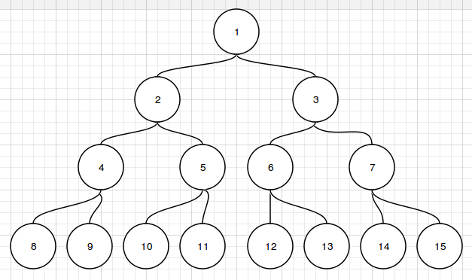
\includegraphics{hw2-1.png}
\item[b)]
Assume that the traversal occurs from left to right.\\
\emph{BFS:} 1,2,3,4,5,6,7,8,9,10,11\\
\emph{DLS:} 1,2,4,8,9,5,10,11\\
\emph{IDS:} 1,1,2,1,2,4,5,3,6,7,1,2,4,8,9,5,10,11\\
\item[c)]
Bidirectional search would work well, since there is only one clearly defined goal state, and the parent of each state is
known. The branching factor down the tree is 2, the branching factor up the tree is 1.
\item[d)]
Yes. Suppose the goal state and initial state were switched, and the tree could only be searched upward instead of downward.
With a branching factor of 1, every edge traversed during the search is guaranteed to be an edge in the solution. If n is the
depth of a binary tree, $\vartheta(n)$ traversals would be required instead of $\vartheta(2^n)$ in the worst case, a dramatic speedup.
\item[e)]
\begin{verbatim}
n = number of goal state
while n > 1:
   n = n/2
   if n == floor(n):
      push 'Left' onto a stack s
   else:
      push 'Right' onto a stack s
   n = floor(n)

while s is not empty:
   pop and output the top of s
\end{verbatim}
\end{enumerate}

\item[\textbf{3.26}]
\begin{enumerate}
\item[a)]
3, because a leaf node that is not in a corner or on a side of the grid has 4 neighboring nodes. Since the root
node is in a corner, each such node in the middle of the grid will have a parent that was not already expanded.
\item[b)]
Conceptually imagine diagonal lines through the grid from upper left to lower right, the first line including
node (0,0); the second line including (0,1) and (1,0); the third line including (2,0),(1,1),(0,2); etc., assuming
$x \ge 2$ and $y \ge 2$. All the nodes on one of lines will first be reachable at the same depth k. This realization
leads to a formula heavily based around the property 
\[
1+2+3+4+ \ldots +n = \frac{n(n+1)}{2}
\]
Now assume that $x \le y$ (x and y can be swapped symmetrically in this formula if $x \ge y$):
\[
number of states(k)=
\begin{cases}
k \le x & \frac{k(k+1)}{2}\\
x < k \le y & \frac{x(x+1)}{2} + x(k-x)\\
k > y & \frac{x(x+1)}{2} + x(y-x) + \frac{x(x-1)}{2} - \frac{(x+y-k)(x+y-k-1)}{2}
\end{cases}
\]
\item[c)]
The maximum number of nodes expanded is unbounded, because the algorithm can become caught in a loop. Say it expands
a node to the north, then to the east, then to the south, then to the west. It can then expand the north node again
and repeat the cycle indefinitely.
\item[d)]
$x \times y - 1$, since no node can be expanded more than once, and since the grid contains $x \times y$ nodes, and
since the goal node does not need to be expanded when it has been reached.
\item[e)]
Yes. The agent can only increment or decrement either the column or the row it is in by 1 per move.
This implies it takes at minimum $|u-x|$ moves to reach the xth column from the uth column, and it takes at minimum
$|v-y|$ moves to reach the yth row from the vth row. So it takes at minimum $|u-x| + |v-y|$ moves to reach the xth
column and yth row from the uth column and vth row.
\item[f)]
Only x+y. A* will only allow the agent to move north or east, since those alternatives are the only ones that lead
to states where h(n) decreases. Thus, it will follow a Manhattan path to the goal.
\item[g)]
Yes. This may cause the Manhattan distance heuristic to \emph{undershoot} the amount of moves that are required to
reach the goal state, but admissible heuristics are allowed to be over-optimistic.
\item[h)]
No. This may cause the Manhattan distance heuristic to \emph{overshoot} the amount of moves that are required to
reach the goal state, which means that it will fail to be admissible.
\end{enumerate}

\item[\textbf{3.27}]
\begin{enumerate}
\item[a)]
States are distinguished by the position of vehicles in the grid. Each of n vehicles can uniquely occupy any of 
$n \times n$ squares. Since each vehicle needs to go to a different destination square, they are distinct. So
there are $P^{n \times n}_n$ different states.
\item[b)]
In the starting state vehicles can only move up, so there are n possible actions in the best case.
In the worst case, however, all vehicles can move in any of the cardinal directions, giving $n \times 4$
possible actions. So the branching factor is $n \times 4$.
\item[c)]
One possibility is use the Manhattan distance from $(n-i+1,n)$ to $(x_i,y_i)$. This is admissible because
a vehicle can only move one square at a time in one of the four cardinal directions, if it is the only
vehicle on the grid.
\[
h(n) = distance_{Manhattan} = |n-i+1-x_i|+n-y_i
\]
\item[d)]
(i) is inadmissible because cars can move 2 squares in one action by hopping if there are multiple cars on the
grid, so in some states the Manhattan distance between a car and its destination would be greater than the number
of moves required to get a car to its destination.

(ii) is admissible. Suppose vehicle i has the largest Manhattan distance of any vehicle from its destination.
If vehicle i cannot hop at any point on the way to its destination, $h_i$ is
no greater than the number of moves required to get vehicle i to its destination, and consequently no greater
than the number of moves required to get all of the vehicles to their destinations. Even if vehicle i can hop
this means that some other vehicle(s) are not at their destination squares and will require at least one move
each to reach their destination squares.

(iii) is admissible because the minimum Manhattan distance of the vehicles is always less than or equal to the
maximum Manhattan distance of the vehicles, which is an admissible heuristic as was just shown.
\end{enumerate}
\end{enumerate}
\end{document}
